% -----------------------------------------------------------------
%		 				 Dynamic Models
% -----------------------------------------------------------------
\begin{tcolorbox}[colback=green!5!white,colframe=green!75!black,title=Linear Time Invariant (LTI) Systems]
with A, B, C, D are matrices
\begin{equation*}
\dot { x } =Ax+Bu \quad y=Cx+Du 
\end{equation*}
\begin{equation*}
G(s)=C{ (sI-A) }^{ -1 }B+D
\end{equation*}

LTI sytems as Input-Output Models
\begin{equation*}
G(S)\, =\, \frac { b_0 + b_1s+...+b_ns^n }{ a_0+a_1s+...+a_{n-1}s^{n-1}+s^n } 
\end{equation*}
\end{tcolorbox}

\begin{tcolorbox}[colback=green!5!white,colframe=green!75!black,title=Deterministic Models:]
$(y(k)=M(k;U,{ x }_{ init },p)$
\textbf{Finite Impulse Response (FIR):}
\begin{equation*}
G(z) = b_0 + b_1z^{-1} + ... + b_{n_b}z^{-n_b} = \frac{b_0z^{n_b} + b_1z^{n_b-1} + ... + b_{n_{b}}}{z^{n_b}+0+...+0}
\end{equation*}
\textbf{Auto Regressive Models with Exogenus Inputs (ARX)}
\begin{equation*}
G(z) = \frac{b_0z^n + b_1z^{n-1} + ... + b_n}{a_0z^n + a_1z^{n-1} + ... + a_n}
\end{equation*}
\end{tcolorbox}

\begin{tcolorbox}[colback=green!5!white,colframe=green!75!black,title=Stochastik Models]
\textbf{Model with measurement Noise:} \\ \(y(k)=M(k;U,{ x }_{ init },p)+\varepsilon(k)\) \\
\textbf{Liniar In the Parameters models (LIP):}
\begin{equation*}
y(k) = \sum_{i= 1}^{d}\theta_i\phi_i(u(k)...,y(k-1),...)+\epsilon(k)
\end{equation*}
$\rightarrow y(k) = \varphi(k)^T\theta + \epsilon(k)$ for $\varphi = (phi_1(\cdot),...,\phi_d(\cdot))$ \\
\textbf{LIP-LTI Models with Equation Errors (ARX)}\\
combining best of two worlds (LTI and LIP)
\begin{equation*}
a_0y(k)+...+a_{n_{a}}y(k-n_a) = b_0u(k)+...+b_{n_{b}}u(k-n_b)+\epsilon(k)
\end{equation*}
\end{tcolorbox}

\begin{tcolorbox}[colback=green!5!white,colframe=green!75!black,title=Model with Input and Output Errors:] 
	\begin{equation*}
	y(k)=M(k;U+{\varepsilon  }_{ N }^{ u },{ x }_{ init },p)+{ { \varepsilon }^{ y } }(k)
	\end{equation*}
\begin{figure}[H]
	\centering
	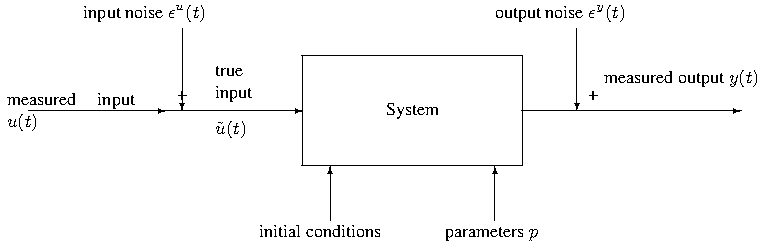
\includegraphics[width=\linewidth]{./model.pdf}
	\label{model}
\end{figure}
\end{tcolorbox}

\begin{tcolorbox}[colback=green!5!white,colframe=green!75!black,title=Pure Output Error (OE) Minimization]
\begin{equation*}
\theta _{ ML } \, =\, arg\, \underset { \theta  }{ min } \, \sum _{ k=1 }^{ N }{ (y(k)-M(k;U,\, x_{ init }\, ,\, p)\, )^{ 2 } }
\end{equation*}

Output Error Minimization for FIR Models
\begin{equation*}
y(k) \, = \, (u(k),\, u(k-1),\, ...,\, u(k-n_{n_b})) \, \cdot \, \theta \, + \, \varepsilon(k)
\end{equation*}
\begin{equation*}
\underset { \theta  }{ min } \sum _{ k=n_{ b }+1 }^{ N }{ (\quad y(k)\, -\, (u(k),\, u(k-1),\, ...,\, u(k-n_{ n_{ b } }))\, \cdot \, \theta \quad )^{ 2 } } 
\end{equation*}

Models with Input and Output Errors
\begin{equation*}
arg \, \underset { \theta  }{ min } \, \sum _{ k-1 }^{ N }{ \frac { 1 }{ { \sigma  }_{ y }^{ 2 } }  } { (y(k)-M(k;U+{ \epsilon  }_{ N }^{ u },{ x }_{ init },p)) }^{ 2 }+\frac { 1 }{ { \sigma  }_{ u }^{ 2 } } { ({ \epsilon  }_{ u }(k)) }^{ 2 }
\end{equation*}
\begin{equation*}
arg \, \underset { \theta  }{ min } \, \sum _{ k-1 }^{ N }{ \frac { 1 }{ { \sigma  }_{ y }^{ 2 } }  } { (y(k)-M(k;\tilde { U } ,{ x }_{ init },p)) }^{ 2 }+\frac { 1 }{ { \sigma  }_{ u }^{ 2 } } { (u(k)-\tilde{ u }(k) ) }^{ 2 }
\end{equation*}
\end{tcolorbox}